\chapter{Theoretische Grundlagen} \label{kap:2}

Das folgende Kapitel legt die theoretischen Grundlagen für die Konzeption des Proof of Concept dar. Es werden Begriffe und Konzepte erläutert, die für das Verständnis der Problemstellung und des entwickelten Ansatzes erforderlich sind. Zunächst wird Barrierefreiheit im Web als Untersuchungsgegenstand definiert (Abschnitt \ref{kap:2.1}), anschließend der Stand automatisierter Barrierefreiheitstools sowie ihre Möglichkeiten und Grenzen (Abschnitt \ref{kap:2.2}). Darauf aufbauend werden dann die besonderen Herausforderungen von Rich-Client-Anwendungen und das Werkzeug Playwright eingeführt (Abschnitt \ref{kap:2.3}). Das Kapitel schließt mit einer Einführung in \acs{LLM}, Modelle und relevante Prompting-Strategien sowie Datenschutzaspekte (Abschnitt \ref{kap:2.4}).

\section{Barrierefreiheit von Webanwendungen} \label{kap:2.1}

\subsection{Begriffsdefinition und Relevanz}

Der Begriff \textit{Web Accessibility}, im Deutschen Web-Barrierefreiheit, bezeichnet nach Definition der \ac{WAI} die Eigenschaft von Webangeboten, von allen Menschen unabhängig von körperlichen, motorischen oder sensorischen Einschränkungen sowie individuellen Fähigkeiten wahrgenommen, bedient und genutzt werden zu können.\footcite[Vgl.][S. 172]{abuaddousWebAccessibilityChallenges2016} Web Accessibility geht jedoch über die reine Wahrnehmbarkeit hinaus und umfasst auch die Bedienbarkeit sowie Nutzbarkeit von Webangeboten.\footcite[Vgl.][]{WAI} Laut Angaben der \ac{WHO} wird geschätzt, dass rund 16\% der Weltbevölkerung mit einer Form von Behinderung leben.\footcite[Vgl.][]{WHO} Diese Zahl umfasst ein breites Spektrum an Einschränkungen, von denen nicht alle die Nutzung digitaler Angebote unmittelbar betreffen. Entscheidend für die Web-Barrierefreiheit sind vor allem visuelle, motorische und kognitive Beeinträchtigungen, die die Wahrnehmung oder Bedienung digitaler Oberflächen erschweren. Damit stellt Barrierefreiheit im Web nicht nur eine technische Herausforderung dar, sondern auch eine zentrale gesellschaftliche Aufgabe zur Gewährleistung digitaler Teilhabe. Das Recht auf barrierefreien Zugang zu Informations- und Kommunikationstechnologien ist seit 2006 in Art. 9 der UN-Behindertenrechtskonvention völkerrechtlich verankert.\footcite[Vgl.][S. 9]{OHCHR}

In der Forschungsliteratur werden vier wesentliche Behinderungsformen unterschieden, die jeweils spezifische Anforderungen an die Gestaltung barrierefreier Webangebote stellen.\footcite[Vgl.][S. 493--494]{ResearchMethodsHumanComputer2017} Für diese Arbeit sind insbesondere zwei Kategorien relevant -- visuelle Beeinträchtigungen und motorische Einschränkungen --, da sie den Großteil der automatisiert prüfbaren \ac{WCAG}-Verstöße betreffen:

\textfett{Visuelle Beeinträchtigungen} umfassen vollständige oder partielle Blindheit sowie Farbfehlsichtigkeit.\footcite[Vgl.][]{gubbi_mohanbabu_context-aware_2024} Betroffene Personen nutzen häufig Screenreader-Software (z.\,B. JAWS, NVDA, VoiceOver), die auf eine korrekte semantische \ac{HTML}-Struktur angewiesen ist.\footcite[Vgl.][S. 5508]{morrisMostItBeing2016} Fehlende Alternativtexte, unzureichende Farbkontraste und fehlende \texttt{aria}-Labels bilden die häufigsten Verstöße in dieser Kategorie\footcite[Vgl.][Erfolgskriterium 1.1.1]{WCAG} und zugleich den primären Erkennungsbereich des in dieser Arbeit entwickelten Systems.

\textfett{Motorische Einschränkungen} betreffen Personen, die konventionelle Eingabegeräte wie Maus oder Touchscreen nicht präzise bedienen können.\footcite[Vgl.][S. 110381--110382]{perezLongitudinalStudyTwo2020} Sie sind auf Tastaturnavigation, Sprachsteuerung oder spezielle assistive Eingabegeräte angewiesen.\footcite[Vgl.][S. 208]{kouroupetroglouAssistiveTechnologiesComputer01} Eine vollständige Bedienbarkeit über die Tastatur ist daher eine zentrale Voraussetzung für barrierefreie Nutzung.\footcite[Vgl.][]{WebAIMKeyboardAccessibility} Für das vorliegende System ist diese Kategorie besonders relevant, da Tastaturfallen und fehlende Fokussteuerung in (React-)Anwendungen häufig erst durch interaktionsbasierte Tests -- etwa mittels Playwright -- aufgedeckt werden können.\footcite[Vgl.][S. 855]{chiou_detecting_2021}

Daneben adressiert die \ac{WCAG} auch auditive und kognitive Beeinträchtigungen; beide erfordern jedoch überwiegend menschliches Urteilsvermögen und entziehen sich weitgehend der automatisierten Prüfung -- sie liegen daher außerhalb des Scopes des vorliegenden \ac{PoC}.\footcite[Vgl.][]{abou-zahra_artificial_2018}

Assistive Technologien -- darunter Screenreader, Bildschirmvergrößerungssoftware und alternative Eingabegeräte -- bilden die technische Voraussetzung für die Nutzung digitaler Angebote durch die genannten Personengruppen.\footcite[Vgl.][]{WAI, abou-zahra_artificial_2018} Ihre Wirksamkeit hängt jedoch unmittelbar davon ab, dass Webanwendungen klar definierte strukturelle und semantische Anforderungen erfüllen.\footcite[Vgl.][S. 82]{morrisonImaginingArtificialIntelligence2017} Die Nichterfüllung dieser Anforderungen führt nicht nur zu einer Beeinträchtigung der betroffenen Personen, sondern kann auch wirtschaftliche und rechtliche Konsequenzen nach sich ziehen.\footcite[Vgl.][S. 864--865]{krok_digital_2024}

\subsection{\ac{WCAG}: Aufbau, Prinzipien und Konformitätsstufen}

Die \acs{WCAG} sind der internationale Standard für barrierefreie Webinhalte und werden vom \ac{W3C} im Rahmen der \ac{WAI} veröffentlicht. Die derzeit maßgebliche Referenzversion ist \ac{WCAG} 2.2, die im Oktober 2023 \ac{WCAG} 2.1 (2018) als aktuelle Referenzversion ablöste.\footcite[Vgl.][]{WCAG2.1,WCAG} \ac{WCAG} 2.2 führt neun zusätzliche Erfolgskriterien ein und berücksichtigt insbesondere kognitive Einschränkungen und mobile Nutzung.\footcites[Vgl.][S. 118]{PolicyPracticeSystematic2025}[Vgl.][]{souzaAccessibilityEvaluationWeb2024} Zu diesen Kriterien gehören konsistentere Fokusindikatoren (2.4.11--2.4.13) und die Vermeidung von Drag-and-Drop-Pflichtinteraktionen (\ac{WCAG} 2.5.7).\footcite[Vgl.][]{WCAG}

Die \ac{WCAG} ist in vier Schichten gegliedert: Prinzipien, Richtlinien, Erfolgskriterien und unterstützende Techniken. Auf oberster Ebene stehen vier grundlegende Prinzipien, 
zusammengefasst im Akronym \textbf{POUR}: \textit{Perceivable} (Wahrnehmbarkeit), \textit{Operable} (Bedienbarkeit), \textit{Understandable} (Verständlichkeit) und \textit{Robust} (Robustheit).\footcite[Vgl.][]{souzaAccessibilityEvaluationWeb2024} Typische Anforderungen sind Alternativtexte für Bilder (1.1.1), ausreichende Farbkontraste (1.4.3) und vollständige Tastaturerreichbarkeit aller Funktionen.\footcite[Vgl.][Abschnitte 1--4]{WCAG}

Die 13 Richtlinien unterhalb der Prinzipien werden durch insgesamt 87 testbare Erfolgskriterien operationalisiert (\ac{WCAG} 2.2; gegenüber 78 in \ac{WCAG} 2.1 kommen neun neue Kriterien hinzu, während SC~4.1.1 als obsolet markiert wird).\footcite[Vgl.][]{WCAG} Jedes Erfolgskriterium ist einer von drei Konformitätsstufen zugeordnet.\footcite[Vgl.][]{fathallah_accessguru_2025} Stufe A umfasst grundlegende Anforderungen, deren Nichteinhaltung bestimmte Nutzergruppen vollständig ausschließt. Stufe AA ist der in Europa gesetzlich geforderte Mindeststandard für öffentliche Stellen und weitere Teile der Privatwirtschaft.\footcite[Vgl.][S. 40, 195 ff.]{kerkmann_barrierefreie_2015} Stufe AAA beschreibt Anforderungen, die nicht für alle Inhalte generell erfüllbar sind. Die vorliegende Arbeit fokussiert sich entsprechend dem gesetzlichen Mindeststandard auf Stufe A und AA.

\begin{figure}[htbp]
  \centering
  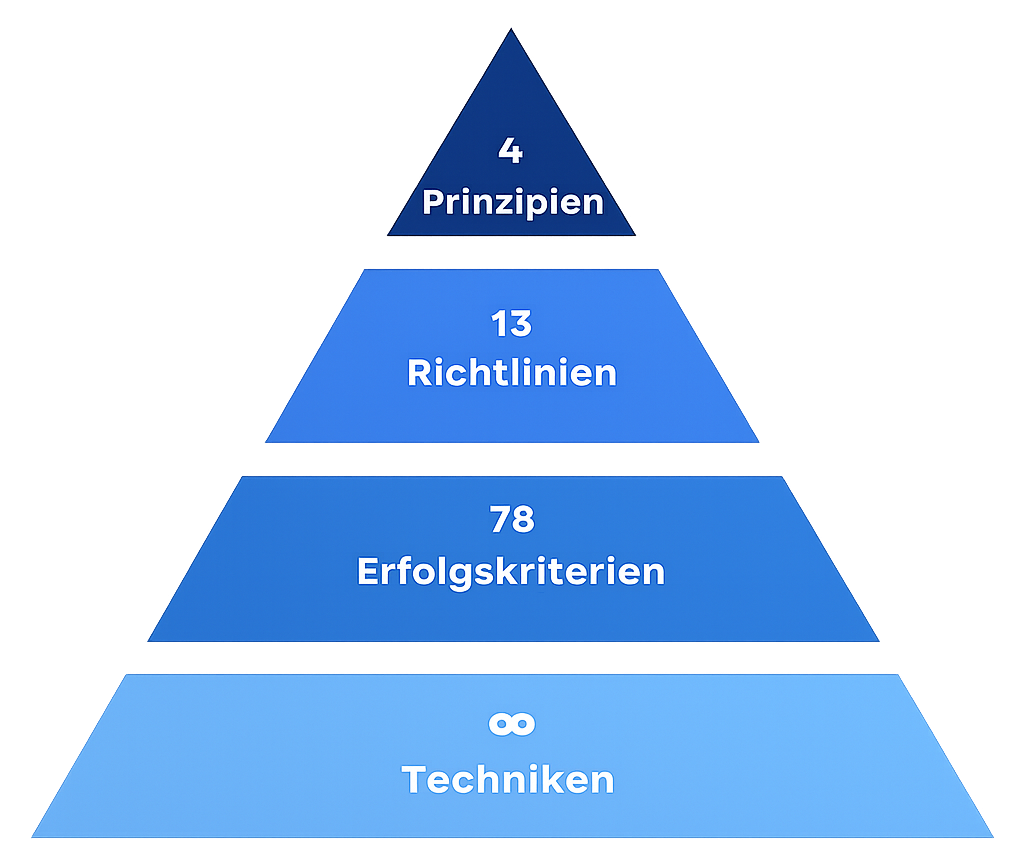
\includegraphics[width=0.4\textwidth]{graphics/WCAG-Dreieck-4-Ebenen.png}
 \caption[\ac{WCAG}-Schichtenmodell]{\ac{WCAG}-Schichtenmodell\protect\footnote{Eigene Abbildung}}
  \label{fig:WCAG-Schichten}
\end{figure}

Die praktische Umsetzung dieser Standards ist trotz ihrer langen Existenz nach wie vor unzureichend.\footcite[Vgl.][S. 297]{bassi_assessment_2025} Die WebAIM-Million-Studie 2025 identifizierte durchschnittlich 56,8 \ac{WCAG}-Fehler pro Seite. Die häufigsten Verstoßkategorien betrafen fehlende Alternativtexte (54,5\%), unzureichende Farbkontraste (80,6\%), fehlende Labels (47,4\%), leere Links (44,6\%) und fehlende Sprachangaben im \ac{HTML} (17,1\%).\footcite[Vgl.][]{WebAIM}

\subsection{Rechtlicher Rahmen}

Auf europäischer Ebene bildet der \acf{EAA} den übergeordneten rechtlichen Rahmen.\footcite[Vgl.][]{EAA} Er verpflichtet die Mitgliedstaaten, Barrierefreiheitsanforderungen für digitale Produkte und Dienstleistungen einheitlich durchzusetzen.

In Deutschland wird der \ac{EAA} durch das \acf{BFSG} in nationales Recht überführt.\footcite[Vgl.][]{BFSG} Das \ac{BFSG} ist seit dem 28. Juni 2025 für privatwirtschaftliche Anbieter verbindlich. Unternehmen mit weniger als zehn Beschäftigten und einem Jahresumsatz unter zwei Millionen Euro sind von bestimmten Pflichten ausgenommen.\footcite[Vgl.][§1 (Anwendungsbereich) und §3 (Barrierefreiheit)]{BFSGGesetz}

Für öffentliche Stellen des Bundes gilt in Deutschland bereits seit 2011 die \acf{BITV} 2.0, die Behörden verpflichtet, ihre Webangebote nach \ac{WCAG} 2.1 auf mindestens Konformitätsstufe AA zu gestalten und zu dokumentieren.\footcite[Vgl.][]{BITV} Die \ac{BITV} 2.0 verweist in ihrer Anlage 1 unmittelbar auf die \ac{WCAG}-Erfolgskriterien und ist damit an deren Weiterentwicklung gekoppelt.

Diese rechtlichen Anforderungen sind für alle betroffenen Organisationen verbindlich -- öffentliche Stellen ebenso wie privatwirtschaftliche Anbieter im Geltungsbereich des \ac{BFSG}. Die \acf{BITBW} als zentrale IT-Dienstleisterin der Landesverwaltung Baden-Württembergs ist davon in besonderem Maße betroffen, da sämtliche von ihr entwickelten oder betriebenen Anwendungen den Anforderungen entsprechen müssen.\footcite[Vgl.][]{BITV} Dies begründet das praktische Interesse an effizienten, automatisierten Methoden der Barrierefreiheitsüberprüfung, wie sie in dieser Arbeit untersucht werden.


\section{Automatisierte Barrierefreiheitsanalyse} \label{kap:2.2}

Trotz klar definierter \ac{WCAG}-Richtlinien wird Barrierefreiheit in der Webentwicklung häufig nur unzureichend umgesetzt. Ein zentraler Grund dafür liegt in den Entwicklungsprozessen moderner Webanwendungen. In vielen Softwareprojekten wird Barrierefreiheit nicht von Beginn an als integraler Bestandteil der Entwicklung berücksichtigt, sondern erst in späten Testphasen oder gar nicht adressiert. Hinzu kommt, dass viele Entwicklerinnen und Entwickler nur begrenztes Wissen über die \ac{WCAG}-Anforderungen besitzen und Accessibility-Aspekte nicht automatisch berücksichtigt werden.\footcite[Vgl.][S. 298]{bassi_assessment_2025} In Kombination mit Zeitdruck und fehlenden automatisierten Prüfverfahren führt dies dazu, dass Accessibility-Probleme häufig erst spät erkannt oder vollständig übersehen werden.\footcite[Vgl.][S. 123]{mowar_accessibility_2024}

\subsection{Klassische Tool-Ansätze} \label{tools}

Für die automatisierte Überprüfung von Webanwendungen auf Barrierefreiheit existiert eine stetig wachsende Zahl von Werkzeugen. Die \ac{WAI} führt in ihrer aktuellen Evaluation-Tool-Liste über 160 Werkzeuge\footcite[Vgl.][]{WAITools}, von denen 84 explizit die \ac{WCAG} 2.1 adressieren.\footcite[Vgl.][]{delnevo_interaction_2024}
Alle gängigen Werkzeuge arbeiten regelbasiert, d.\,h. sie prüfen den \ac{DOM} einer geladenen Seite anhand eines vordefinierten Regelkatalogs gegen bekannte Verstoßmuster.\footcites[Vgl.][]{kodithuwakku_assessing_2025}[][3:9]{manca_transparency_2023}
Das \acf{DOM} ist eine vom Browser erzeugte, baumartige Objektstruktur, die den \ac{HTML}-Code einer Webseite als hierarchische Struktur aus Elementknoten repräsentiert und über Programmierschnittstellen von Skripten und Analysewerkzeugen zugänglich macht.\footcite[Vgl.][]{Robie}

Zu den meistgenutzten automatisierten Barrierefreiheitstools gehören:
\begin{itemize}
    \item \textbf{axe-core}, entwickelt von Deque Systems, hat sich als Standardlösung für die automatische Integration von Accessibility-Tests in Entwicklungspipelines etabliert.\footcite[Vgl.][]{axe}
    \item \textfett{WAVE} (WebAIM) bietet visuelle Browser-Extensions, die Fehler direkt in der gerenderten Seitenansicht annotieren.\footcite[Vgl.][]{WAVE}
    \item \textfett{Lighthouse} ist in die Chrome-DevTools integriert und kombiniert Accessibility-Testing mit Performance- und SEO-Analysen.\footcite[Vgl.][]{Lighthouse}
    \item \textfett{IBM Equal Access Checker} und \textfett{ARC Toolkit} (TPGi) runden das Spektrum verbreiteter Werkzeuge ab.
\end{itemize}

Der typische Output solcher Werkzeuge ist ein strukturierter Violation Report, bei dem jedem erkannten Verstoß eine Bezeichnung, Beschreibung und ein Schweregrad zugewiesen wird (bei axe-core: minor, moderate, serious, critical) sowie, falls möglich, ein \ac{HTML}-Ausschnitt des betroffenen Elements.\footcites[Vgl.][]{kodithuwakku_assessing_2025}[][]{axe} Dieser standardisierte Output bildet in der vorliegenden Arbeit die Grundlage für die erste Stufe der Datenpipeline.

\subsection{Grenzen bestehender Tools} \label{kap:grenzen Tools}

Trotz ihrer weiten Verbreitung weisen regelbasierte Accessibility-Tools fundamentale Grenzen auf. Diese lassen sich in drei Kategorien einteilen: begrenzte Regelabdeckung, semantische Blindheit und fehlende Dynamik.

Die Regelabdeckung der Werkzeuge ist erheblich geringer als oftmals angenommen. Kodithuwakku und Wickramaarachchi zeigen, dass selbst die leistungsfähigsten untersuchten Tools lediglich 21\% aller \ac{WCAG}-Tests automatisiert abdecken können (vgl. Tabelle \ref{tab:tool_evaluation}).\footcite[Vgl.][]{kodithuwakku_assessing_2025} Die in der Tabelle ausgewiesenen Werte CER und ICR messen davon abweichende Dimensionen: CER beschreibt, welcher Anteil der tatsächlich gemeldeten Befunde korrekt ist (Präzision), während ICR angibt, wie viele der vorhandenen Probleme vom Tool gefunden wurden (Recall). Für Tastaturzugänglichkeit und auditive Barrieren lag die Erkennungsrate in ihrer Studie bei null Prozent; hinzu kommt eine hohe Rate an \textit{False Positives}.\footcite[Vgl.][]{kodithuwakku_assessing_2025} Bassi et al. kommen zu dem Ergebnis, dass das beste verfügbare Einzeltool (\textfett{ARC Toolkit}) nur 26\% der \ac{WCAG}-Tests abdeckt.\footcite[Vgl.][S. 298]{bassi_assessment_2025}%
% KÜRZUNG: Fussnote zur eingeschränkten Vergleichbarkeit der beiden Studien auf einen Satz gekürzt.
\footnote{Die Vergleichbarkeit beider Studien ist eingeschränkt, da unterschiedliche Testkorpora und Methodiken verwendet werden; die übereinstimmende Kernaussage -- regelbasierte Tools decken nur einen Bruchteil aller prüfbaren \ac{WCAG}-Kriterien ab -- ist dennoch robust.}
Die Kombination mehrerer Tools in einem Ensemble verbessert die Abdeckung, beseitigt das strukturelle Problem jedoch nicht vollständig. Pool zeigt, dass selbst ein Ensemble aus acht gleichzeitig eingesetzten Tools, darunter auch \textfett{axe-core}, \textfett{WAVE} und \textfett{Qualweb}, erhebliche Lücken hinterlässt: jedes einzelne Tool erkennt mindestens sieben Violations exklusiv, die von keinem anderen Tool gefunden werden.\footcite[Vgl.][]{pool_testaro_2023} Manca et al. stellen zudem fest, dass von elf untersuchten Werkzeugen lediglich drei explizit auf ihre Erkennungslücken hinweisen.\footcite[Vgl.][S. 4]{manca_transparency_2023}


\begin{table}[htbp]
\centering
\small
\begin{tabular}{lcccc}
\toprule
\textbf{Tool} & \textbf{True Positives} & \textbf{False Positives} & \textbf{CER (\%)} & \textbf{ICR (\%)} \\
\midrule
Lighthouse & 17 & 16 & 52.94 & 15.92 \\
WAVE & 16 & 12 & 35.29 & 14.65 \\
SiteImprove & 23 & 18 & 47.06 & 19.75 \\
axe & 15 & 10 & 52.94 & 15.29 \\
Accessibility Insights & 24 & 19 & 47.06 & 15.29 \\
A11y & 6 & 8 & 23.53 & 3.82 \\
Includia Accessibility Checker & 33 & 31 & 41.18 & 21.02 \\
\bottomrule
\end{tabular}
\caption[Erkennungsleistung von Accessibility-Tools]{Vergleich der Erkennungsleistung verschiedener Accessibility-Prüfwerkzeuge.\footcite[Entnommen aus][]{kodithuwakku_assessing_2025} CER beschreibt den Anteil korrekt erkannter Verstöße im Verhältnis zu allen gemeldeten Verstößen, während ICR den Anteil tatsächlich vorhandener Accessibility-Probleme misst, die vom jeweiligen Tool erkannt werden.}
\label{tab:tool_evaluation}
\end{table}

Das gravierendste Defizit liegt in der \textbf{semantischen Blindheit} der Werkzeuge.\footcite[Vgl.][]{fathallah_accessguru_2025} Regelbasierte Tools können lediglich prüfen, ob ein Accessibility-Attribut vorhanden ist, nicht aber, ob der Inhalt dem richtigen Zweck dient. Ein Bild mit dem Alternativtext \textit{image} oder \textit{IMG\_0042.jpg} wird von allen Tools als regelkonform eingestuft, obwohl dieser Text für Screenreader-Nutzende keinen Mehrwert bietet. \textbf{Ma11y}, ein Mutation-Testing-Framework für Accessibility, hat dieses Problem empirisch quantifiziert: Bei der systematischen Injektion von 25 gezielten Defekten in reale Webanwendungen erkannten die sechs ausgewählten Tools semantische Verstöße nur zu 26\% und syntaktische Verstöße zu 54\% -- im Durchschnitt blieb damit nahezu die Hälfte aller injizierten Defekte unentdeckt.\footcite[Vgl.][S. 108]{tafreshipour_ma11y_2024}

Ein weiteres strukturelles Problem ist die \textfett{fehlende Dynamik} der Analyse. Viele Tools analysieren ausschließlich den initial geladenen \ac{DOM}-Zustand einer Seite.\footcite[Vgl.][]{fathallah_accessguru_2025} Barrieren, die erst durch Nutzerinteraktionen entstehen -- etwa beim Öffnen eines Modalfensters, beim Aktivieren eines Dropdown-Menüs oder beim Erscheinen einer Fehlermeldung -- bleiben dabei unsichtbar. Hinzu kommt, dass alle Violation Reports generischer Natur sind: Sie beschreiben das Problem auf der Ebene des gerenderten \ac{DOM}, ohne Bezug zur Quellcodestruktur der geprüften Anwendung herzustellen.\footcite[Vgl.][]{delnevo_interaction_2024}

\subsection{Taxonomie der Verstöße: syntaktisch, semantisch, Layout} \label{Taxonomie}
Um Barrierefreiheitsverstöße systematisch analysieren und gezielt adressieren zu können, wird in dieser Arbeit eine dreiteilige Taxonomie zugrunde gelegt, die auf Fathallah et al. zurückgeht (vgl. Abbildung~\ref{fig:taxonomie_verstoesse}).\footcite[Vgl.][]{fathallah_accessguru_2025}

\begin{itemize}
    \item \textfett{Syntaktische Verstöße} bezeichnen Fälle, in denen ein erforderliches Accessibility-Element vollständig fehlt oder formal falsch gebildet ist.\footcite[Vgl.][S. 102]{tafreshipour_ma11y_2024} Ein typisches Beispiel ist ein fehlendes \texttt{alt}-Attribut an einem \texttt{<img>}-Element. Diese Kategorie ist für regelbasierte Tools am besten prüfbar, da die Verletzung rein struktureller Natur ist.\footcite[Vgl.][S. 569 ff.]{Flanagan_2020}
    \item \textfett{Semantische Verstöße} liegen vor, wenn Accessibility-Attribute zwar vorhanden sind, ihren Zweck aber inhaltlich verfehlen.\footcite[Vgl.][]{WCAG} Ein Bild mit dem Alternativtext \textit{Bild} oder ein Link mit dem Text \textit{hier klicken} sind typische Beispiele. Da die Bewertung solcher Verstöße Sprachverständnis und Kontextwissen erfordert, bilden sie das primäre Anwendungsfeld für \ac{LLM}-basierte Analysen.\footcite[Vgl.][FSE101:2]{he_enhancing_2025}
    \item \textbf{Layout-Verstöße} betreffen visuelle Barrieren, insbesondere unzureichende Farbkontraste\footcite[Vgl.][Erfolgskriterium 1.4.3]{WCAG} und fehlende oder schwer erkennbare Fokusindikatoren.\footcite[Vgl.][Erfolgskriterium 2.4.7--2.4.13]{WCAG} Einige dieser Verstöße können algorithmisch geprüft werden; andere erfordern ein kontextuelles visuelles Urteil.
\end{itemize}


\begin{figure}[htbp]
\centering
\begin{tikzpicture}[
  catbox/.style={
    rectangle, rounded corners=3pt,
    minimum width=4.2cm, minimum height=1.1cm,
    draw=#1!60, fill=#1!8, line width=0.8pt,
    font=\bfseries\small, align=center
  },
  exbox/.style={
    rectangle, rounded corners=2pt,
    minimum width=4.2cm,
    draw=#1!30, fill=white, line width=0.5pt,
    font=\scriptsize, align=left, text=black,
    inner sep=5pt
  },
  detectbox/.style={
    rectangle, rounded corners=2pt,
    minimum width=4.2cm, minimum height=0.7cm,
    draw=#1!40, fill=#1!5, line width=0.5pt,
    font=\scriptsize\itshape, align=center, text=black
  },
]

% Column 1: Syntaktisch
\node[catbox=blue] (syn) {Syntaktisch};
\node[exbox=blue, below=4mm of syn] (syn-ex) {%
  \textbullet~Fehlendes \texttt{alt}-Attribut\\
  \textbullet~\texttt{<table>} ohne \texttt{<th>}\\
  \textbullet~Fehlender \texttt{aria-label}%
};
\node[detectbox=blue, below=3mm of syn-ex] (syn-det) {Regelbasiert pr\"ufbar};

% Column 2: Semantisch
\node[catbox=orange, right=8mm of syn] (sem) {Semantisch};
\node[exbox=orange, below=4mm of sem] (sem-ex) {%
  \textbullet~\texttt{alt="Bild"}\\
  \textbullet~Label: \textit{Eingabe}\\
  \textbullet~Linktext: \textit{hier klicken}%
};
\node[detectbox=orange, below=3mm of sem-ex] (sem-det) {Sprachverst\"andnis n\"otig};

% Column 3: Layout
\node[catbox=teal, right=8mm of sem] (lay) {Layout};
\node[exbox=teal, below=4mm of lay] (lay-ex) {%
  \textbullet~Unzureichender Kontrast\\
  \textbullet~Fehlender Fokusindikator\\
  \textbullet~Eingeschr\"ankte Zoomf\"ahigkeit%
};
\node[detectbox=teal, below=3mm of lay-ex] (lay-det) {Teils algorithmisch pr\"ufbar};

% Header
\node[above=8mm of sem, font=\small\bfseries] (title) {Taxonomie der Barrierefreiheitsverst\"o\ss e};

% Detection difficulty arrow
\draw[-{Stealth[length=3mm]}, line width=1pt, black]
  ([yshift=-3mm]syn-det.south west) -- ([yshift=-3mm]lay-det.south east)
  node[midway, below=1mm, font=\scriptsize, text=black] {Zunehmende Komplexit\"at der Erkennung};

\end{tikzpicture}
\caption{Taxonomie der Barrierefreiheitsverst\"o\ss e nach Fathallah et al. mit Beispielen und Erkennungscharakteristik je Kategorie}
\label{fig:taxonomie_verstoesse}
\end{figure}

\FloatBarrier
\section{Rich-Client-Webanwendungen und Testautomatisierung}\label{kap:2.3}
\subsection{Charakteristika und Abgrenzung}

Der Begriff \textfett{Rich-Client-Webanwendung} bezeichnet Webanwendungen, bei denen ein Großteil der Anwendungslogik und Darstellungssteuerung clientseitig im Browser ausgeführt wird.\footcite[Vgl.][]{React} Im Gegensatz zu klassischen serverseitig gerenderten Anwendungen werden bei einer \ac{SPA} nach dem initialen Laden des \ac{HTML}-Rahmens ausschließlich Daten zwischen Client und Server ausgetauscht, wobei die Darstellung durch clientseitige Skriptsprachen wie JavaScript oder TypeScript direkt im Browser durch Manipulation des \ac{DOM} gesteuert wird.\footcite[Vgl.][]{ReactRender} Die zunehmende Komplexität solcher Anwendungen ist in Anhang~\ref{anhang:complexity} veranschaulicht.

React, ein von Meta entwickeltes JavaScript-Framework, ist derzeit der dominante Ansatz zur Entwicklung solcher Anwendungen. Laut Stack Overflow Developer Survey 2025 wird React von 44,7\% aller befragten Entwicklerinnen und Entwickler eingesetzt.\footcite[Vgl.][]{Stack_Overflow_2025}
\begin{figure}[htbp]
  \centering
  \includegraphics[width=0.5\textwidth]{graphics/react.png}
  \caption[Framework Popularity über die letzten Jahre]{Framework Popularity über die letzten Jahre\footcite[Entnommen aus][]{262588213843476FrontendFrameworksPopularity}}
  \label{fig:react}
\end{figure}

Für die Barrierefreiheitsanalyse sind zwei Architekturmerkmale von React besonders relevant: Erstens werden Anwendungslogik und Darstellung in wiederverwendbaren \textbf{Komponenten} gekapselt, deren Kommunikation über \textbf{Props} (unveränderliche Eingabeparameter) und internen \textbf{State} (veränderlicher Zustand) erfolgt.\footcite[Vgl.][]{React} Zweitens wird die Darstellung der Komponenten mithilfe der Syntaxerweiterung \ac{JSX} (bzw. TSX bei Verwendung von TypeScript) definiert, die \ac{HTML}-ähnliche Strukturen direkt in JavaScript- oder TypeScript-Code einbettet.\footcite[Vgl.][]{baiVirtualDom2022}

\subsection{Herausforderungen für die Barrierefreiheitsprüfung} \label{Herausforderungen}

Komponentenbasierte Frameworks wie React, Vue oder Angular teilen bestimmte Architekturmerkmale, die die Barrierefreiheitsanalyse grundsätzlich erschweren.\footcite[Vgl.][S. 110]{tafreshipour_ma11y_2024} Da die vorliegende Arbeit eine React-Anwendung als Untersuchungsgegenstand verwendet, werden die folgenden Herausforderungen anhand von React konkretisiert; sie gelten in ähnlicher Form jedoch auch für andere komponentenbasierte Frameworks.

Erstens entstehen viele Barrierefreiheitsprobleme \textbf{zustandsabhängig},
wie bereits in Kapitel \ref{kap:grenzen Tools} erläutert. Ein Modalfenster kann sich nach einem Klick öffnen, ohne den Tastaturfokus korrekt zu verwalten. Ebenso kann eine Fehlermeldung nach dem Absenden eines Formulars erscheinen, ohne über eine ARIA-Live-Region programmatisch angekündigt zu werden. Auch ein Dropdown-Menü kann für Tastaturnutzende nicht navigierbar sein. All diese Probleme sind im initialen Seitenzustand nicht vorhanden und damit für statische Analysewerkzeuge unsichtbar.\footcites[Vgl.][S. 5--6]{he_enhancing_2025}[Vgl.][Erf.-krit. 2.4.3 \& 4.1.3]{WCAG} In React wird diese Problematik durch das State-Management verstärkt: Zustandsänderungen lösen ein erneutes Rendering einzelner Komponenten aus, wobei sich die Accessibility-Eigenschaften des resultierenden \ac{DOM} je nach State unterscheiden können.

Zweitens besteht eine \textbf{Diskrepanz zwischen Quellcode und gerendertem \ac{DOM}}. In React werden Benutzeroberflächen in \ac{JSX}/TSX definiert; der im Browser gerenderte \ac{DOM} ist das Ergebnis der React-Laufzeitumgebung, die diese Definitionen in \ac{DOM}-Elemente übersetzt. Ein Accessibility-Tool analysiert den gerenderten \ac{DOM}, nicht aber den Quellcode, aus dem er hervorging.\footcite[Vgl.][S. 31]{fernandesEvaluatingAccessibilityWeb2012} Für Entwicklerinnen und Entwickler ist jedoch der Quellcode der relevante Interventionspunkt.\footcite[Vgl.][]{fathallah_accessguru_2025} Ein konkretes Beispiel: Eine React-Komponente \texttt{IconButton} rendert im \ac{DOM} ein \texttt{<button>}-Element mit einem \texttt{<svg>}-Icon, jedoch ohne sichtbaren Text und ohne \texttt{aria-label}. axe-core meldet den Verstoß \textit{button-has-visible-text} mit dem \ac{HTML}-Ausschnitt \texttt{<button class="btn-icon">...</button>} -- ohne Hinweis darauf, dass die Ursache in der Datei \texttt{IconButton.tsx} liegt, wo das \texttt{aria-label}-Prop nicht weitergereicht wird.

Drittens erschwert die \textbf{Komponentenabstraktion} die Ursachenanalyse: Eine wiederverwendbare Komponente mit einem Accessibility-Problem manifestiert sich im gerenderten \ac{DOM} an jeder Stelle, an der sie eingesetzt wird. Accessibility-Tool-Reports melden jeden einzelnen Treffer separat, ohne den Bezug zur gemeinsamen Quellkomponente herzustellen, deren einmalige Korrektur alle Treffer beseitigen würde.\footcite[Vgl.][]{abou-zahra_artificial_2018}

\subsection{Playwright als Testautomatisierungswerkzeug}

Um diese dynamischen Zustände automatisiert reproduzierbar testen zu können, werden Werkzeuge zur Browserautomatisierung benötigt.

Playwright ist ein von Microsoft entwickeltes Open-Source-Framework für die End-to-End-Test\-automatisierung von Webanwendungen.\footcite[Vgl.][]{playwright} Es ermöglicht die automatisierte Steuerung von Chromium, Firefox und WebKit über eine einheitliche \ac{API} und führt Anwendungen in einem echten Browser-Kontext aus, sodass JavaScript-Ausführung, clientseitiges Rendering und dynamische \ac{DOM}-Manipulationen vollständig nachgebildet werden.

Für die Barrierefreiheitsanalyse ist Playwright aus mehreren Gründen besonders geeignet. Erstens kann es durch programmierte Interaktionen -- Klicks, Formularausfüllungen, Tastatureingaben, Hover-Aktionen -- gezielt verschiedene Anwendungszustände auslösen.\footcite[Vgl.][]{playwright}
Zweitens bietet Playwright mit \texttt{@axe-core/playwright} eine direkte Integration der axe-core-Bibliothek: Nach jeder Interaktion kann unmittelbar eine vollständige axe-Prüfung des aktuellen \ac{DOM}-Zustands angestoßen werden.\footcite[Vgl.][]{axe}

Verschiedene Forschungsarbeiten nutzen diese Integration bereits erfolgreich für die Barrierefreiheitsanalyse dynamischer Webanwendungen (vgl. Kapitel~\ref{kap:3}). In der vorliegenden Arbeit dient Playwright als zentrales Werkzeug der Detection-Phase: Es löst definierte Interaktionssequenzen aus, erfasst die resultierenden \ac{DOM}-Zustände und stößt axe-core-Prüfungen an, deren strukturierter \acs{JSON}-Output als erster Input für die \ac{LLM}-Analysepipeline dient.

\section{\ac{KI}-Assistenzsysteme für Softwareanalyse und Handlungsempfehlungen}\label{kap:2.4}

Innerhalb der \ac{KI}-Forschung haben sich \ac{LLM}s als besonders leistungsfähige Klasse von Systemen für sprachbasierte Aufgaben etabliert.\footcite[Vgl.][S. 22]{russellArtificialIntelligenceModern2021} Für die vorliegende Arbeit sind sie relevant, weil sie sowohl Code verstehen als auch natürlichsprachige Handlungsempfehlungen generieren können.

\subsection{Grundlagen: Large Language Models}

\ac{LLM}s sind neuronale Netzwerke, die auf extrem großen Datensätzen mit dem Ziel trainiert werden, das nächste Token einer Textsequenz vorherzusagen.\footcite[Vgl.][S. 5--6]{brynjolfssonGenerativeAIWork2025} Die zugrunde liegende Architektur ist der Transformer, der ausschließlich auf Attention-Mechanismen basiert und rekurrente sowie konvolutionale Netze in der Sequenzmodellierung ablöst.\footcite[Vgl.][]{vaswani2023attentionneed} Durch dieses Training auf massiver Datenbasis entstehen Modelle, die komplexe Sprachstrukturen, semantische Zusammenhänge und Formen logischen Schlussfolgerns abbilden. Für den Zugriff auf externes Wissen werden häufig \textit{Embedding}-basierte Retrieval-Methoden verwendet (Vektorraumsuche), die in \ac{RAG}-Systemen zentral sind.\footcite[Vgl.][S. 2--3]{lewisRetrievalAugmentedGenerationKnowledgeIntensive2021} Zu den bekanntesten Modellfamilien zählen GPT-4o (OpenAI), Claude (Anthropic) und LLaMA (Meta).\footcite[Vgl.][]{anthropic2026claude, openai2023gpt4, touvron2023llama2} Entscheidend für den Anwendungskontext dieser Arbeit sind die sogenannten \textit{emergent abilities} dieser Modelle: Fähigkeiten wie Code-Generierung, mehrsprachige Übersetzung und kontextuelles Schlussfolgern, die ab einer bestimmten Modellgröße ohne explizites Training auftreten.\footcite[Vgl.][S. 2]{wei2022emergent}

Im Kontext der Barrierefreiheitsanalyse bieten \ac{LLM}s gegenüber regelbasierten Tools vier wesentliche Vorteile:\footcite[Vgl.][]{fathallah_accessguru_2025}
\begin{itemize}
    \item Sie verfügen über ein Sprachverständnis, das die Bewertung semantischer Inhalte ermöglicht -- etwa die Beurteilung, ob ein Alternativtext den Bildinhalt tatsächlich beschreibt.\footcite[Vgl.][]{tafreshipour_ma11y_2024}
    \item Sie können Code generieren und transformieren, wodurch konkrete Handlungsempfehlungen abgeleitet werden können.\footcites[Vgl.][S. 3]{touvron2023llama2}
    \item Sie können große Mengen an Text analysieren und strukturieren.\footcite[Vgl.][S. 298]{bassi_assessment_2025}
    \item Sie verarbeiten Kontext und können die Bedeutung eines Elements im Zusammenhang der Gesamtseite beurteilen.\footcite[Vgl.][]{fathallah_accessguru_2025}
\end{itemize}

Diesen Stärken stehen bekannte Schwächen gegenüber:
\begin{itemize}
    \item \ac{LLM}s können halluzinieren, also plausibel klingende Ausgaben erzeugen, die jedoch faktisch falsch sind.\footcite[Vgl.][1:2]{huangSurveyHallucinationLarge2025}
    \item Sie sind von einem \textit{Knowledge-Cutoff} betroffen: Dem Modell sind nach diesem Stichtag veröffentlichte Informationen nicht bekannt.\footcites[Vgl.][S. 7]{System_Card}[][1:9--10]{huangSurveyHallucinationLarge2025} Dies gilt auch für das in dieser Arbeit eingesetzte Modell qwen2.5-coder:7b\footcite[Vgl.][]{hui2024qwen25coder}, das keine danach veröffentlichten \ac{WCAG}-Änderungen oder Bibliotheks-Updates kennt.
    \item Bei identischer Eingabe erzeugen sie nicht notwendigerweise identische Ausgaben (\textit{Nicht-Determinismus}).\footcites[Vgl.][]{OpenAI_Developers}[Vgl.][]{anthropic2026claude}
    \item Die generierten Inhalte können Verzerrungen (\textit{Bias}) aus den Trainingsdaten übernehmen.\footcite[Vgl.][S. 614--615]{benderDangersStochasticParrots2021}
\end{itemize}

Eine für die vorliegende Arbeit zentrale Frage ist, ob diese Fähigkeiten auch bei kleineren, lokal ausführbaren Modellen in ausreichendem Maße vorhanden sind. Alle in Kapitel~\ref{kap:3} untersuchten Systeme -- AccessGuru, GenA11y, ACCESS -- setzen GPT-4o ein, ein Modell mit geschätzt über 200 Milliarden Parametern und Zugang zu umfangreichen Cloud-Ressourcen.\footcites[Vgl.][]{fathallah_accessguru_2025}[Vgl.][FSE101:10]{he_enhancing_2025}[Vgl.][S. 7]{huang_access_2024} Lokal ausführbare Modelle der 7B-Klasse verfügen über deutlich weniger Parameter und damit potenziell über ein eingeschränkteres Sprachverständnis und schwächere Reasoning-Fähigkeiten. Ob ein solches Modell semantische Accessibility-Verstöße zuverlässig erkennen kann, ist empirisch bislang nicht belegt und wird in der vorliegenden Arbeit als explizite Forschungsfrage adressiert. Die Begründung der konkreten Modellauswahl erfolgt in Kapitel~\ref{kap:4.4}.

\subsection{Prompt-Engineering-Strategien} \label{Prompt}

Die Qualität der Ausgaben eines \ac{LLM} hängt maßgeblich von der Formulierung der Eingabe -- dem sogenannten Prompt -- ab. Prompt-Engineering bezeichnet die systematische Gestaltung dieser Eingaben, um die Ausgabequalität zu maximieren.\footcite[Vgl.][S. 4]{schulhoff2024promptreport} Im Folgenden werden die für diese Arbeit relevanten Strategien beschrieben, die in Kapitel \ref{kap:6} als Grundlage für das Prompt-Design des \ac{PoC} dienen.

\begin{itemize}
    \item \textbf{Zero-Shot Prompting} bezeichnet die direkte Anfrage ohne Beispiele oder Kontextinformationen. Das Modell nutzt ausschließlich sein vortrainiertes Wissen. Diese Strategie ist einfach umzusetzen, erzielt bei komplexen Aufgaben wie der Barrierefreiheitsanalyse jedoch häufig unzureichende Ergebnisse.\footcites[Vgl.][S. 4]{brown2020gpt3fewshot}[Vgl.][]{njifenjou_role-play_2024}
    \item \textbf{Few-Shot Prompting} ergänzt den Prompt um eine kleine Anzahl von Beispielen (Input-Output-Paaren), die dem Modell das erwartete Ausgabeformat und die inhaltlichen Erwartungen verdeutlichen. Dieser Ansatz verbessert die Konsistenz und Präzision der Ausgaben erheblich, erfordert jedoch sorgfältig ausgewählte Beispiele.\footcite[Vgl.][S. 5]{brown2020gpt3fewshot} Abbildung~\ref{fig:fewshot} vergleicht Zero-Shot- und Few-Shot-Prompting.
    \item \textbf{Chain-of-Thought Prompting (CoT)} veranlasst das Modell, seinen Lösungsweg Schritt für Schritt zu erklären, bevor es zur finalen Antwort gelangt. Dieses explizite Reasoning reduziert nachweislich Halluzinationen bei komplexen Schlussfolgerungen.\footcites[Vgl.][S. 2]{wei2022chainofthought}[][]{fathallah_accessguru_2025}
    \item \textbf{ReAct-Prompting} kombiniert Reasoning (Re) und Action (Act) iterativ: Das Modell wechselt zwischen Denk- und Handlungsschritten, etwa durch das Einbeziehen von Tools und Zwischenergebnissen. Huang et al. demonstrieren, dass ReAct-Prompting bei der automatisierten Barrierefreiheitskorrektur (\textfett{ACCESS}) mit einem Severity Score Reduction von 51,3\% alle anderen verglichenen Strategien übertrifft.\footcites[Vgl.][S. 5]{huang_access_2024}[][S. 1]{yao2022react}
    \item \textbf{Role-Play Prompting} weist dem Modell eine Expertenrolle zu, die seine Ausgaben in Richtung domänenspezifischen Wissens lenkt. Ein Prompt, der dem Modell die Rolle eines \glqq erfahrenen Barrierefreiheitsexperten und React-Entwicklers\grqq{} zuweist, verbessert nachweislich die Qualität accessibility-spezifischer Ausgaben.\footcites[Vgl.][]{fathallah_accessguru_2025}[][]{njifenjou_role-play_2024}[][S. 6, 12]{schulhoff2024promptreport}
    \item \textbf{Metacognitive Prompting} fordert das Modell auf, die eigene Ausgabe in einem zweiten Schritt zu reflektieren und zu bewerten, bevor diese finalisiert wird.\footcites[Vgl.][]{wangMetacognitivePromptingImproves2024}[][S. 8--9]{schulhoff2024promptreport} In Verbindung mit Corrective Re-Prompting -- einer Technik, bei der fehlerhafte Ausgaben dem Modell mit einer Fehlerbeschreibung zurückgespielt werden -- ermöglicht dieser Ansatz eine iterative Qualitätssteigerung. Fathallah et al. belegen, dass Corrective Re-Prompting in \textfett{AccessGuru} den Violation Score Decrease von 0,72 auf 0,84 verbessert.\footcite[Vgl.][]{fathallah_accessguru_2025}
\end{itemize}

\begin{figure}[htbp]
  \centering
  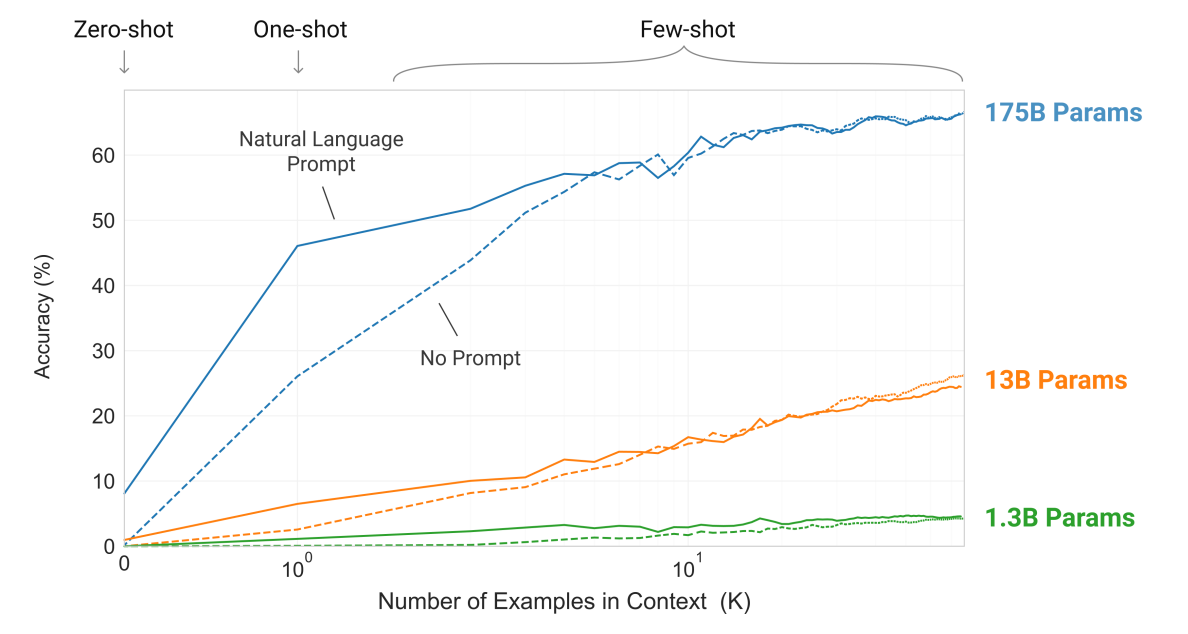
\includegraphics[width=0.7\textwidth]{graphics/fewshot.png}
  \caption[Zero-Shot und Few-Shot Prompting im Vergleich]{Zero-Shot und Few-Shot Prompting im Vergleich\footcite[Entnommen aus][]{brown2020gpt3fewshot}}
  \label{fig:fewshot}
\end{figure}


\subsection{\acs{RAG} und Fine-Tuning als Erweiterungsansätze}

\textbf{\acf{RAG}} erweitert den Prompt zur Laufzeit mit thematisch passenden Dokumenten aus einer externen Wissensbasis und könnte im Accessibility-Kontext aktuelle \ac{WCAG}-Kriterien unabhängig vom Trainings-Cutoff abrufbar machen.\footcite[Vgl.][S. 1--2]{lewisRetrievalAugmentedGenerationKnowledgeIntensive2021} \textbf{Fine-Tuning} bezeichnet das domänenspezifische Training auf einem aufgabenspezifischen Datensatz; für den Kontext der \ac{BITBW} wäre insbesondere ein Fine-Tuning auf \ac{BITV}-spezifischen Anforderungen denkbar.\footcite[Vgl.][S. 90]{silvestreSystemsOpportunitiesLLM2025} Beide Ansätze liegen außerhalb des Scopes dieser Arbeit und werden im Ausblick (Abschnitt~\ref{sec:fazit_ausblick}) aufgegriffen.

\subsection{Datenschutz bei \ac{KI}-gestützten Accessibility-Services} \label{datenschutz}

Der Einsatz von \ac{LLM}s im Kontext öffentlicher Verwaltungen wirft spezifische Datenschutzfragen auf. Webanwendungen der öffentlichen Verwaltung verarbeiten häufig personenbezogene Daten -- etwa in Formularseiten, die persönliche Angaben von Bürgerinnen und Bürgern erfassen. Werden diese Seiten für eine \ac{KI}-gestützte Accessibility-Analyse an externe \ac{LLM}-\ac{API}s übermittelt, ist die Wahrung der Datenschutzgarantien fraglich.

Die \ac{DSGVO} schreibt vor, dass personenbezogene Daten nur auf Basis einer Rechtsgrundlage und unter Wahrung der Grundsätze der Zweckbindung und Datenminimierung verarbeitet werden dürfen.\footcite[Vgl.][]{dsgvo2016} Die Übermittlung von \ac{HTML}-Quellcode der produktiven Anwendung, der im schlimmsten Fall personenbezogene Daten als Attributwerte enthalten kann, an externe \ac{API}-Dienste wie die OpenAI \ac{API} oder die Anthropic \ac{API} ist ohne explizite Rechtsgrundlage und einen Auftragsverarbeitungsvertrag nach Art. 28 \ac{DSGVO} für öffentliche Verwaltungen in Deutschland problematisch.\footcite[Vgl.][Art. 28]{dsgvo2016}

Als Lösungsansatz wird in dieser Arbeit ein Lokal-First-Prinzip verfolgt: Das \ac{KI}-Assistenzsystem soll ohne externe \ac{API}-Aufrufe betreibbar sein, indem lokal ausführbare Open-Source-Modelle -- etwa Modelle der LLaMA-Familie oder Mistral -- eingesetzt werden.\footcite[Vgl.][]{touvron2023llama2} Damit bleiben sämtliche Analyse- und Codedaten innerhalb der eigenen Infrastruktur. Diese Anforderung prägt sowohl die nicht-funktionalen Anforderungen (Kapitel \ref{kap:4}) als auch die Architekturentscheidungen (Kapitel \ref{kap:6}) dieser Arbeit.

Die in diesem Kapitel erarbeiteten theoretischen Grundlagen -- das normative Fundament der \ac{WCAG}, die empirisch belegten Grenzen regelbasierter Tools, die Besonderheiten von React-Anwendungen sowie die Möglichkeiten und Grenzen von \ac{LLM}s und des Prompt Engineerings -- bilden den konzeptionellen Rahmen für die im folgenden Kapitel aufgearbeitete Forschungsliteratur sowie für die anschließend dargestellte Methodik.